\documentclass[12pt]{article}
\usepackage{graphicx}
\usepackage[spanish]{babel}
%opening

\author{Victor Hugo Pacheco Fonseca}

\begin{document}
	\title{\Huge{\textbf{Moogle Project}}}
	\author{\textit{Victor Hugo Pacheco Fonseca}}
	\date{16 de julio del 2023}
	
	\begin{figure}
		\centering
		
\includegraphics[scale=0.4]{imagen}
	\end{figure}
	\maketitle
	\newpage
	
	\section{\Huge {Introducción}}	
	
	Moogle es un buscador como cualquier otro. Su tarea es encontrar archivos .txt correspondientes a la búsqueda realizada en los documentos  dentro de una carpeta que sirve de base de datos.El programa está dividido en 2 componentes fundamentales: MoogleServer que se encarga de la interfaz gráfica, donde se recibe la consulta y se muestran los resultados y MoogleEngine una biblioteca de clases donde esta implementado casi todo el algoritmo de funcionamiento del programa. Este proyecto esta orientado a explicar como se debe ejecutar el programa y se da una explicación de la composición y el funcionamiento de MoogleEngine.   
	
	
	\newpage
	\section{\Huge {Ejecución del Proyecto}}
	Para ejecutar el programa de forma adecuada se debe seguir los siguentes pasos: 
	\begin{enumerate}
		\item Debe copiar los documentos en lo que se quiere buscar en la carpeta 'Content', en formato .txt
		\item Luego desde carpeta raíz ejecutar el comando según el sistema operativo con que se está
		trabajando
		
	\end{enumerate}
	Para brindar mayor exactitud a la consulta, el proyecto cuenta con un corrector de palabras, por
	si el usuario escribió incorrectamente alguna palabra.
	\section{\Huge{Modelo vectorial}}
	Para la realización de la búsqueda fue utilizado el cálculo de Modelo Vectorial. Este se utiliza
	para ver que tan parecido son 2 documentos mediante el cálculo de que tan relevante es una
	palabra en un documento, a lo que se le denomina TF-IDF, en el cual:
	
	TF=$\frac{w}{d}$  y IDF=$\log$($\frac{n}{q}$)
	
	donde:
	
	w = Cantidad de veces que aparece una palabra en un documento.
	
	d = Cantidad de palabras en total que contiene el documento.
	
	n = Cantidad de documentos en total. 
	
	q = Cantidad de documentos en los que aparece la palabra.
	
	
	
	\section{\Huge{Funcionalidad del proyecto} }
	\subsection{\textit{Procesamiento de los documentos}}
	Al iniciar el programa , se llama al metodo InsertWords de la clase Vocabulario que se encarga
	de leer los documentos y guardarlos cada uno en un array de Listas. Luego recorre cada
	documento y a cada palabra le crea un objeto de tipo WordInfo donde se guarda la cantidad de
	veces que parece la palabra en cada documento, si la palabra no había aparecido antes se añade
	al vocabulario.
	\subsection{\textit{Creación de los vectores documento}}
	Luego se llama al método InsertDoc de la clase Vocabulario. Este se encarga de hacer un objeto
	tipo Document para cada documento (vector documento),en donde se guarda el título del mismo
	y un diccionario donde se almacena cada palabra (sin repetir) con su respectivo TF-IDF, luego d
	terminado el objeto se añade a un array de Document.
	\subsection{\textit{Procesamiento de la Query}}
	Al usuario introducir la Query se crea un array de string con cada palabra de la misma. Luego se
	comprueba si alguna palabra introducida no se encuentra en el Vocabulario, en caso de no
	encontrarse alguna(por ejemplo si el usuario escribió una palabra mal) , se llama al metodo
	Suggestions de la clase SearchResult el cual se encarga de encontrar la palabra más parecida a
	través del método  LevenshteinDistance.
	
	LevenshteiDistance esta basada en un algoritmo d programación el cual se encarga d comparar
	dos palabras y retornar la cantidad d cambios que se necesita para transformar una a otra.Estos cambios pueden ser:
	
	Agregar una letra.
	
	Eliminar una letra.
	
	Cambiar una letra por otra.
	
	Luego de procesada la Query se crea un objeto tipo Document (vector consulta) para la misma y
	se guarda el TF-IDF de cada palabra al igual que con los documentos.
	\subsection{\textit{Similitud entre los vectores y la Query}}
	Luego se procede a calcular el score de cada documento creando un objeto tipo SearchItem para
	cada uno y se almacenan en un array. De ello se encarga el método SimCos de la clase
	SearchItem. Este se basa en la medida del coseno del ángulo entre cada vector Document
	almacenado en la clase Vocabulario y el vector Consulta. De esta manera se calcula el valor de
	similitud. Si no hay coincidencia alguna entre los componentes de los vectores se dice que estos
	son ortogonales o lo que es igual a que su coincidencia es cero. La similitud máxima se alcanza
	cuando todos los componentes de los vectores son iguales, en este caso la función del coseno
	obtiene su máximo valor, que es uno.
	Luego ordenamos el array de forma decreciente en función de cada score calculado.Ver figura \ref{fig:cos}.
	\begin{figure}[h!]
		\centering
		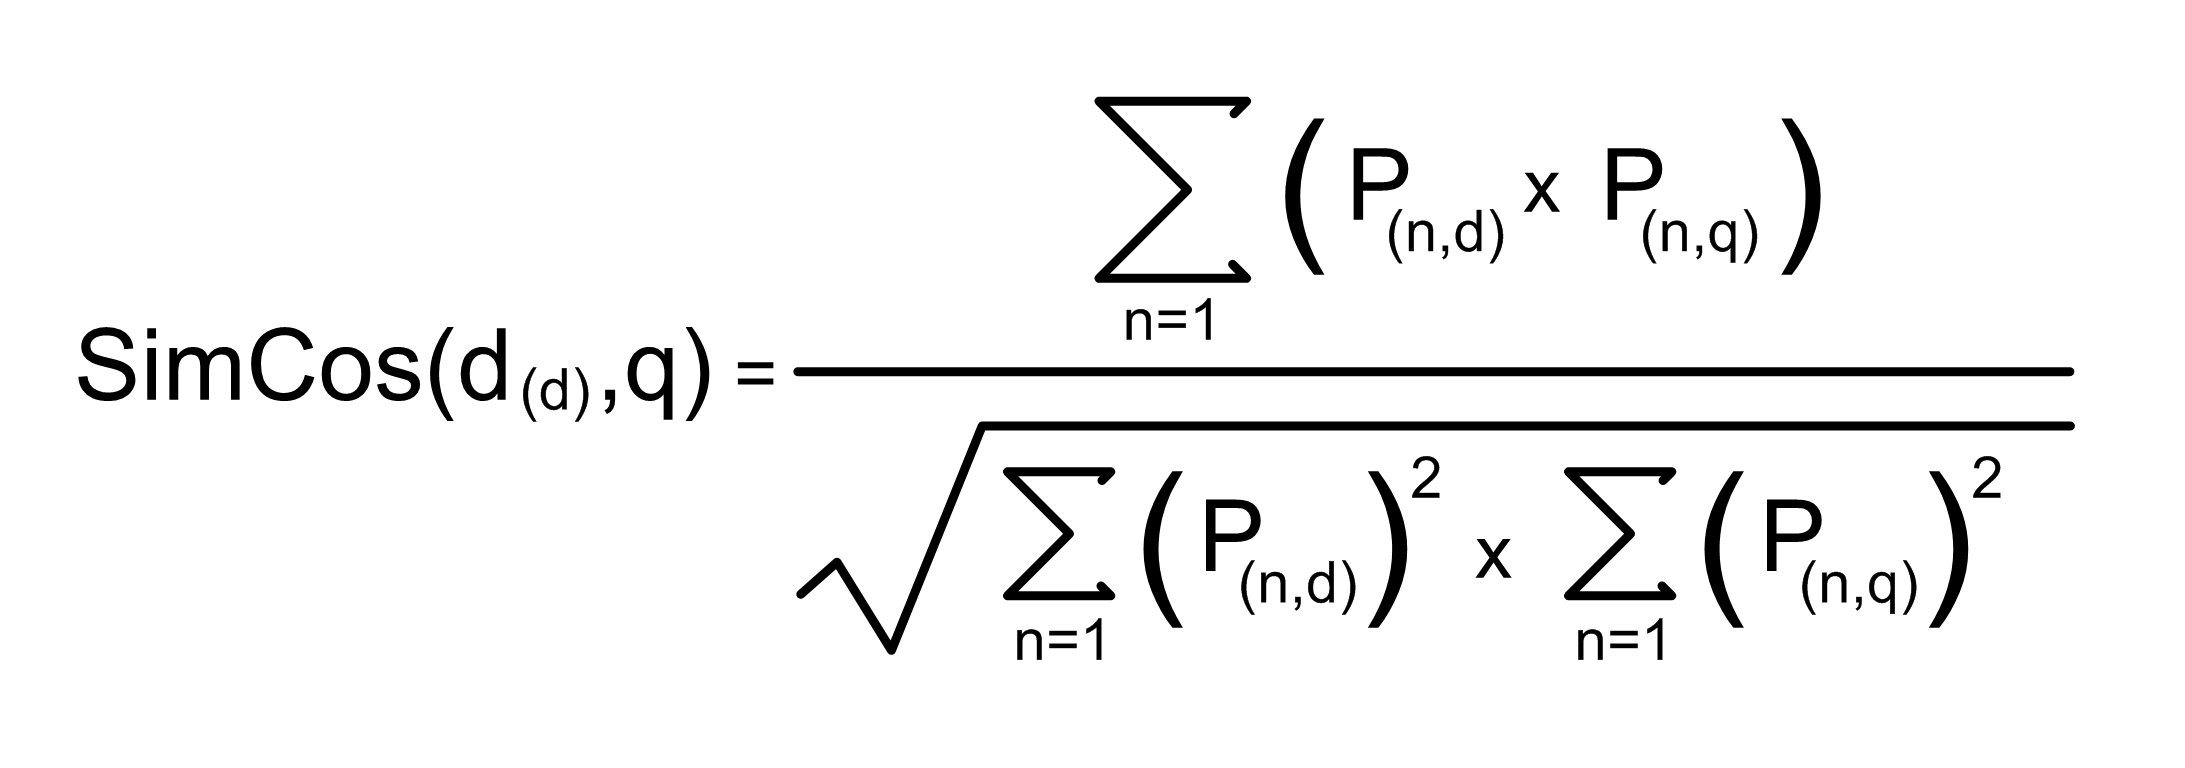
\includegraphics[scale=0.4]{simcos}
		\caption{Fórmula para el cálculo de la similaridad del coseno}
		\label{fig:cos}
	\end{figure}
	
	\subsection{\textit{Snippet}}
	Para la obtención del snippet se llama al metodo GetSnippet de la clase SnippetClass. Este busca
	cuales es la palabra con más peso de la Query y retorna un pedazo del documento a partir de la
	primera aparición de dicha palabra. Por último se construye un objeto tipo tipo Search Results con el array de SearchItems obtenidos
	anteriormente y en caso de no haber encontrando una palabra de la consulta en el Vocabulario
	se devuelve su palabra más similar.
	
	\section{Concluciones}
	asdadsgdgsdyfsghrtheuetr
	
	
\end{document}
